\documentclass[a4paper, 11pt]{article}  
\usepackage{fullpage} % changes the margin
\usepackage[brazilian]{babel}
\usepackage[utf8]{inputenc}
\usepackage[T1]{fontenc}
\usepackage{graphicx}

\begin{document}

\noindent
\large\textbf{Apps Controle Alimentar e Nutricional} \hfill \textbf{Marcos Cordeiro de Brito Jr} \\
Prof. Nizam Omar
Disciplina: Inteligência Artificial

\begin{center}
\huge\textbf{Resenha}
\end{center}

\section{Calorie Mama}
\begin{center}
    
\includegraphics[width=6cm]{calories_mama.png}
\end{center} 

\textsf{Calorie Mama App} é um aplicativo que utiliza Inteligência Artificial para identificar itens de alimento com rapidez e precisão. Utilizando \textit{machine learning}, o usuário utiliza a câmera do celular para tirar fotos e o aplicativo calcula a quantidade de calorias em cada refeição.

Ao utilizar o app pela primeira vez, o usuário precisa imputar idade, sexo, altura e peso para calcular o IMC e criar a rotina de exercícios e dietas para alcançar um objetivo.  Entre as opções disponíveis, o usuário pode escolher entre perder peso, fazer mais exercícios, consumir menos calorias, beber mais água ou dormir melhor.

Inserindo as informações diariamente dos alimentos consumidos, quantidade de exercícios que foram feitas, quilometragem de caminhadas ou corridas, automaticamente é calculado e mostrado quanto falta para o usuário atingir seus objetivos.

O aplicativo ainda traz um atrativo de compartilhamento de fotos e progresso em sua própria rede social. Todas essas opções estão disponíveis na opção free. Na opção premium é possível acessa um plano de dieta padronizado ao objetivo, lembrete das refeições e acompanhamento das atividades cardíacas. 

\begin{center}
    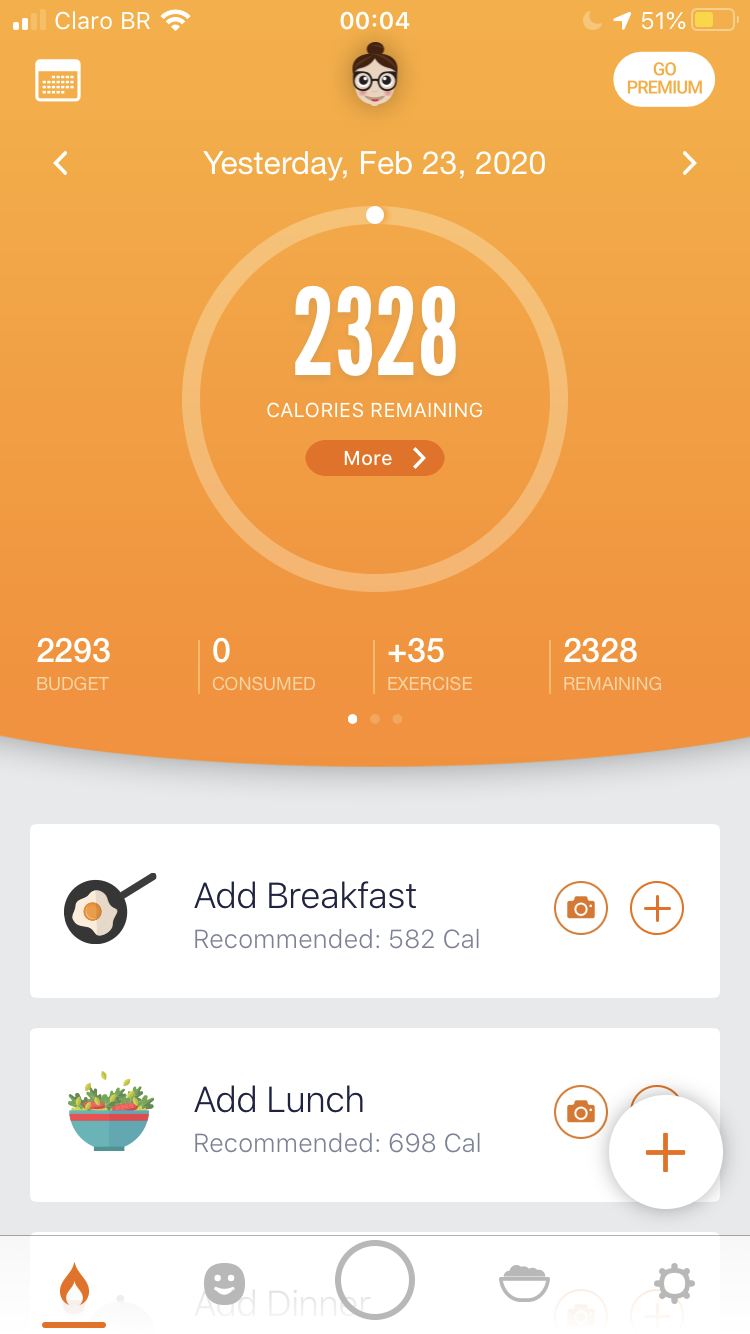
\includegraphics[width=5cm]{calories_mama_print.png}
\end{center} 
\newpage

\section{FitGenie}
\begin{center}
    \includegraphics[width=5cm]{fitgenie.png}
\end{center} 

O \textsf{FitGenie} é um aplicativo mais simples e direto. Seu objetivo é apenas controlar a quantidade de proteínas,  carboidratos e gordura consumidas pelo usuário.

Após inserir as informações básicas para o cálculo de IMC, o usuário informa quantos quilos quer perder e, através das calorias dos alimentos consumidos durante o dia, o aplicativo diz se esta dentro ou fora do seu objetivo. Para facilitar, o aplicativo identifica os alimentos através da leitura de código de barras.

Para ter acesso a mais funcionalidades como plano customizado de refeições, receitas ou objetivos macros personalizados, o usuário precisará assinar a opção premium.

\begin{center}
    \includegraphics[width=5cm]{fitgenie_print.jpeg}
\end{center} 
\newpage

\section{Lifesum}
\begin{center}
    
\includegraphics[width=5cm]{lifesum.png}
\end{center} 

Muito parecido com o FitGenie, \textsf{Lifesum} utiliza das informações básicas de IMC do usuário para traçar o plano de perda de peso baseado na rotina de exercícios e calorias consumidas. A atualização das informações também são feitas de forma manual ou com auxílio da leitura de código de barras dos produtos consumidos.

O diferencial do Lifesum em relação o concorrente anterior, esta nas funcionalidades do plano pago. Através de um questionário de 41 perguntas, o aplicativo faz uma análise das informações para traçar um plano customizado visando o objetivo desejado. Neste plano também são disponibilizados receitas saudáveis com baixo consumo de calorias para ajudar na dieta do usuário.

\begin{center}
    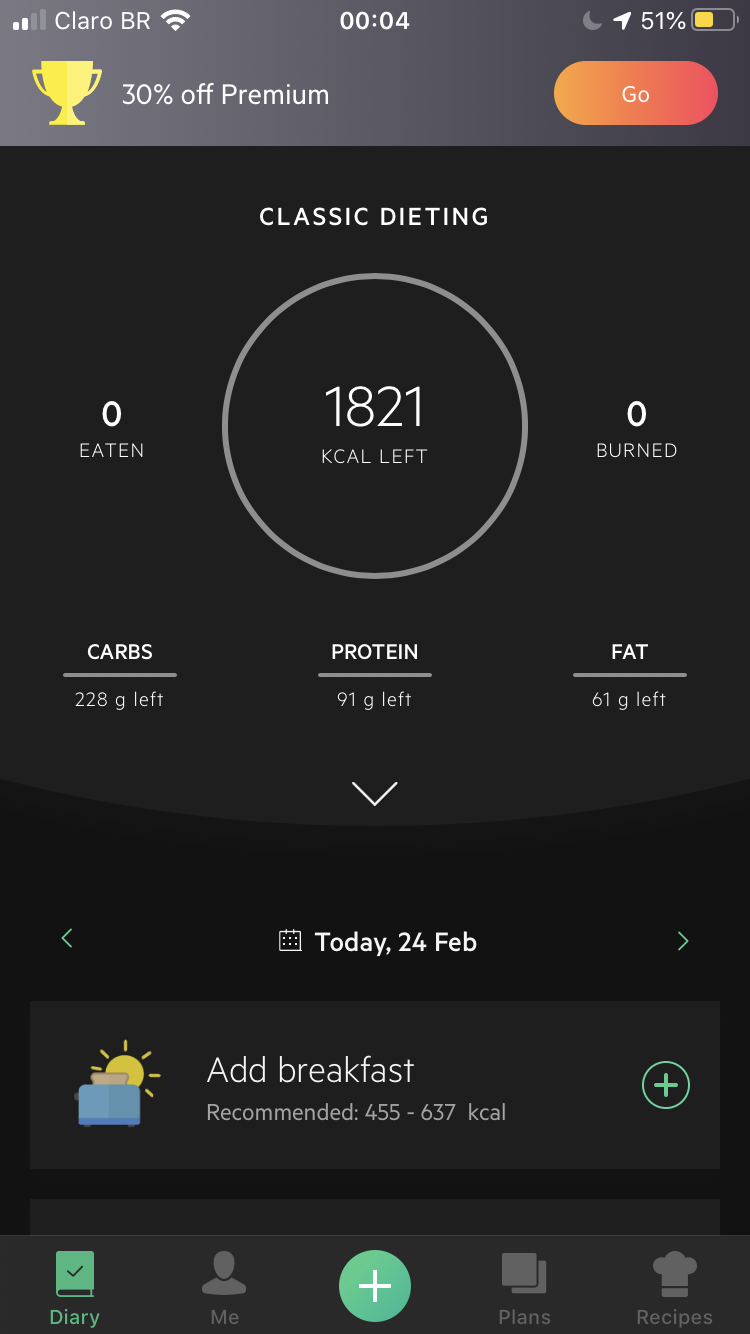
\includegraphics[width=5cm]{lifesum_print.png}
\end{center} 

\end{document}